\chapter{Implementation}
This chapter focus mainly about the software implementation for semi-automated detection of sanitization, authentication and declassification errors in UML state Charts. Used Eclipse xtext to develop source code editor, Eclipse xtend to develop source code generator, YAKINDU SCT editor for modeling C/C++ programs as UML statchart and extended static analysis engine named smtcodan using Java, Graphics2D and Jframe. 

\section{Overview of System Architecture}

A system architecture or systems architecture is the conceptual model that defines the structure, behavior and more views of a system. An architecture description is a formal description and representation of a system, organized in a way that supports reasoning about the structures and behaviors of the system.

It can be said that the system architecture is (similar to the one of a building architecture)  a global model of this system consisting of:
\begin{itemize}
	\item   a structure
	\item	properties (of various elements involved)
	\item	relationships (between various elements)
	\item	behaviors and dynamics
	\item	multiple views of the system (complementary and consistent).
\end{itemize}

System Architecture is based on 9 fundamental principles:
\begin{itemize}
	\item The objects of the reality are modelled as systems
	\item A system can be broken down into a set of smaller subsystems, which is less than the whole system
	\item A system must be considered in interaction with other systems
	\item A system must be considered through its whole lifecycle
	\item System can be linked to another through an interface, which will model the properties of the link
	\item A system can be considered at various abstraction levels, allowing to consider only relevant properties and behaviors
	\item A system can be viewed according to several layers (usually three: its sense, its functions, and its composition)
	\item A system can be described through interrelated models with given semantics (properties, structure, states, behaviors, datas, etc)
	\item A system can be described through different viewpoints corresponding to various actors concerned by the system.
\end{itemize}

The architecture of our system is given below:
\begin{figure}[htbp]
	\centering
	\makebox[\textwidth]{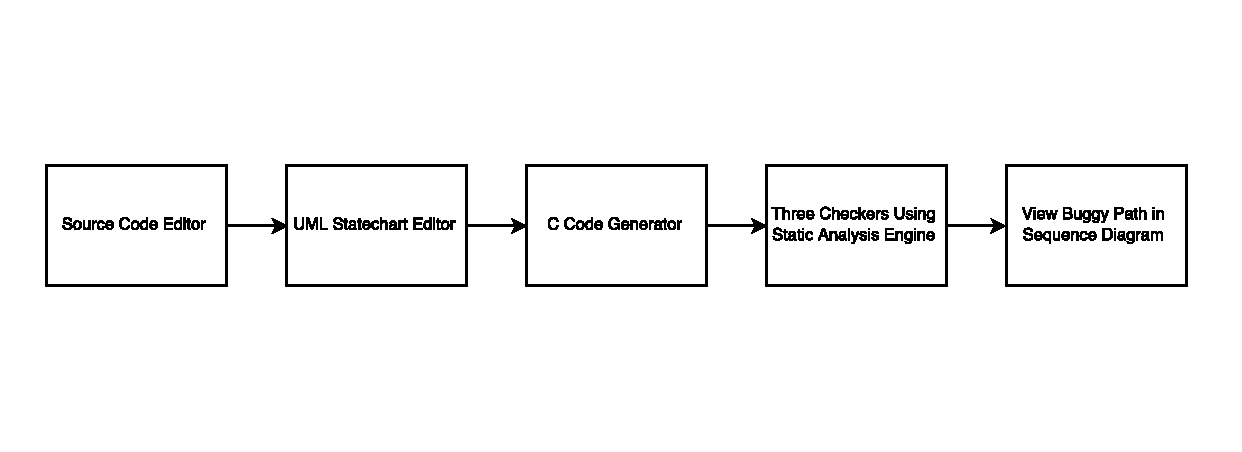
\includegraphics[width=\textwidth]{styles/system_architecture.pdf}}
	\caption{System Overview}
\end{figure}

Figure 4.1 depicts the complete system architecture. First, the source code editor is developed using Eclipse Xtext. By this editor one can easily annotate the source code of C/C++. Even it is possible to annotate C/C++ header files. For information flow vulnerabilities detection in C/C++ code this annotation technique has chosen which is easy to extend and backward compatible. This editor has developed as an Eclipse plug-in. If this plug-in exist in eclipse then user can easily annotate C/C++ source code files and header files by pressing the keys ctrl+space in keyboard. Then for modeling purpose open source tool Yakindu SCT editor \cite{ref_15_yakindu:sct} has chosen to model the C/C++ code into state charts to detect the bug during design stage of software development life-cycle. Inside the Yakindu SCT editor the annotation language grammar has also included using Eclipse Xtext. So, that user can easily annotate the state charts to detect the information flow vulnerabilities. Afterwards the C code generator has extended inside the Yakindu SCT editor using Eclipse Xtend. After modeling the C code files in Yakindu SCT editor user can easily generate the code using C code generator. Through this generator two files will be generated. One file has .c extension and another file has .h extension. Inside those files annotation has also included. Those annotations are helpful to detect the information flow errors. After generating the code files using static analysis engine named \enquote{smtcodan} three checkers have included to detect authentication, declassification and sanitization function missing vulnerabilities. Inside the static analysis engine according to the requirements new modules are added. Then to view the buggy path in sequence diagram a sequence diagram generator has created. That is the end of complete system architecture of this system. 


\section{The Grammar of Annotation Language}

The goal of the annotation language is to convey library-specific information to the compiler in a simple declarative manner. While it's clear that more sophisticated specifications could support more sophisticated optimizations, our goal is to show that a few simple annotations can enable many useful optimizations. Simplicity is important because we expect our language users to be library experts who do not necessarily have expertise in compilers or formal specifications.

An annotation is metadata (like a comment, explanation, presentational markup) attached to text, image, or other data. Often, annotations refer to a specific part of the original data.Markup languages like XML and HTML annotate text in a way that is syntactically distinguishable from that text. They can be used to add information about the desired visual presentation, or machine-readable semantic information. If annotations are to be machine-readable, they must have a well-defined syntax, and if a tool's checks are to be meaningful, the annotations also need a well-defined semantics. Quite a few specification languages have been defined over the past several decades; 

A special case is the Java programming language, where annotations can be used as a special form of syntactic metadata in the source code. Classes, methods, variables, parameters and packages may be annotated. The annotations can be embedded in class files generated by the compiler and may be retained by the Java virtual machine and thus influence the run-time behavior of an application. It is possible to create meta-annotations out of the existing ones in Java.

The "annotate" function (also known as "blame" or "praise") used in source control systems such as Git, Team Foundation Server and Subversion determines who committed changes to the source code into the repository. This outputs a copy of the source code where each line is annotated with the name of the last contributor to edit that line (and possibly a revision number). This can help establish blame in the event a change caused a malfunction, or identify the author of brilliant code.

For example, Standard Annotation Language or SAL \cite{ref_51_microsoft:sal} is a meta-language that can help static analysis tools, such as analyze switch in Visual Studio 2005 Team System and Visual Studio 2005 Team Edition for Developers, find bugs including security bugs in your C or C++ code at compile time.
Using SAL is relatively easy. You simply add annotations to your function prototypes that describe more contextual information about the function being annotated. This can include annotations to function arguments and to function return values. The initial focus of SAL is to annotate functions that manipulate read and write buffers. In Windows Vista we are annotating all appropriate functions before the product is released to customers to help us find bugs as early as possible.

\begin{table}
	\centering
	\begin{tabular}{|l|c|p{5cm}|}
		\hline
		Category  & Parameter Annotation & Description  \\
		\hline
		
		Input to called function        & \_In\_k  		   & Data is passed to the called function, and 
		is treated as read-only\\
		\hline
		
		Input to called function, and output to caller        & \_Inout\_ & Usable data is passed into the function 
		and potentially is modified. \\ \hline
		Output to caller        & \_Out\_ & The caller only provides space 
		for the called function to write to. 
		The called function writes
		data into that space. \\
		\hline
		
		Output of pointer to caller         & \_Outptr\_  & Like Output to caller. The value that's returned by the called function is a pointer.\\ 	\hline
			
	\end{tabular}
	\caption{SAL-four basic kinds of parameters}
	\label{table:four basic kinds of parameters}
\end{table}

These four basic annotations can be made more explicit in various ways. By default, annotated pointer parameters are assumed to be required ,they must be non-NULL for the function to succeed. The most commonly used variation of the basic annotations indicates that a pointer parameter is optional, if it's NULL, the function can still succeed in doing its work.These annotations help identify possible uninitialized values and invalid null pointer uses in a formal and accurate manner. Passing NULL to a required parameter might cause a crash, or it might cause a "failed" error code to be returned. Either way, the function cannot succeed in doing its job.

The main benefit of SAL is that you can find more bugs with just a little bit of upfront work. The process of adding SAL annotations to existing code can also find bugs as the developer questions the assumptions previously made about how the function being annotated works. By this as a developer adds annotations to a function, she must think about how the function works in more detail than simply assuming it was written correctly. This process finds assumption flaws. Any bugs found in SAL annotated functions tend to be real bugs, not false positives, which has the benefit of speedier bug triage and code fixes.

In this research, annotation language is developed using Eclipse xtext \cite{ref_17_xtext:grammar}. The goal is to overcome the challenge of not being able to detect implicit and explicit information flow bugs in UML state charts and C code. That's why an annotation language has chosen
which can be used to annotate UML state charts and code by inserting information flow
restrictions during two software development phases (design
and coding). Our insight is that the same annotation language
can be used to add information flow constraints to UML state
charts and code in order to detect information flow errors. The grammar of annotation language is represented as in Extended Backus Naur Form (EBNF) in Figure \ref{language grammar}. The following type face conventions were used: Italic font for non-terminals, bold typewriter font for literal terminals including keywords.\\
 
 \begin{figure}[ht!]
 	\centering
 	\begin{tabular}{lll}
 		
 		\footnotesize                       
 		\textit{Ann\_Lang}           &\footnotesize $::=$         &\footnotesize HeaderModel*;       \\ \\
 		
 		\footnotesize
 		\textit{H\_Model}            &\footnotesize $::=$         &\footnotesize \textit{S\_L\_Anno};       \hfill ;single line comment rule   \\     
 		&\footnotesize $\ \vert $    &\footnotesize \textit{M\_L\_Anno};       \hfill ;multi line comment rule    \\ 
 		&\footnotesize $\ \vert $    &\footnotesize \textit{Func\_Ann};       \hfill ;function declaration rule  \\ 
 		&\footnotesize $\ \vert $    &\footnotesize \textit{Attr\_Def};        \hfill ;variable declaration rule  \\ \\
 		\footnotesize  	
 		\textit{S\_L\_Anno}          &\footnotesize $::=$         &\footnotesize \textbf{"//@ @function "},    Func\_Type,              [\textbf{H} $\ \vert $  \textbf{L}];     \\
 		&\footnotesize $\ \vert $    &\footnotesize \textbf{"//@ @parameter "},   p\_Name,  Sec\_Type, Var\_Type,    [\textbf{H} $\ \vert $  \textbf{L}];    \\
 		&\footnotesize $\ \vert $    &\footnotesize \textbf{"//@ @variable "},    v\_Name,  Sec\_Type,     [\textbf{H} $\ \vert $  \textbf{L}];    \\
 		&\footnotesize $\ \vert $    &\footnotesize \textbf{"//@ @preStep "},     pr\_s\_Name,             [\textbf{H} $\ \vert $  \textbf{L}];    \\
 		&\footnotesize $\ \vert $    &\footnotesize \textbf{"//@ @postStep "},    po\_s\_Name,             [\textbf{H} $\ \vert $  \textbf{L}];    \\ \\   
 		\footnotesize            
 		\textit{M\_L\_Anno}          &\footnotesize $::=$         &\footnotesize [\textbf{"/*@ "}],  ["* "],  Func\_Ann,  (\textbf{" @*/"}) \\
 		&\footnotesize $\ \vert $    &\footnotesize ("*"), [" "]*, (\textbf{"@*/"});                  \\ \\
 		\footnotesize        
 		\textit{Func\_Ann}           &\footnotesize $::=$         &\footnotesize \textbf{"@function "},    Func\_Type,              [\textbf{H} $\ \vert $  \textbf{L}];     \\
 		&\footnotesize $\ \vert $    &\footnotesize \textbf{"@parameter "},   p\_Name,  Sec\_Type, Var\_Type,    [\textbf{H} $\ \vert $  \textbf{L}];    \\
 		&\footnotesize $\ \vert $    &\footnotesize \textbf{"@preStep "},     pr\_s\_Name,             [\textbf{H} $\ \vert $  \textbf{L}];    \\
 		&\footnotesize $\ \vert $    &\footnotesize \textbf{"@postStep "},    po\_s\_Name,             [\textbf{H} $\ \vert $  \textbf{L}];    \\ \\                                        
 		\footnotesize                       
 		\textit{Func\_Type}          &\footnotesize $::=$        &\footnotesize \textbf{authentication};\\
 		&\footnotesize $\ \vert $ &\footnotesize \textbf{declassification}; \\
 		&\footnotesize $\ \vert $    &\footnotesize \textbf{sanitization};     \\
 		&\footnotesize $\ \vert $    &\footnotesize \textbf{sink};             \\
 		&\footnotesize $\ \vert $    &\footnotesize \textbf{source};           \\
 		&\footnotesize $\ \vert $    &\footnotesize \textbf{trust\_boundary};  \\ \\
 		\footnotesize                       
 		\textit{Sec\_Type}           &\footnotesize $::=$         &\footnotesize \textbf{confidential}; \\
 		&\footnotesize $\ \vert $    &\footnotesize \textbf{source};    \\ \\
 		\footnotesize                       
 		\textit{Var\_Type}           &\footnotesize $::=$         &\footnotesize \textbf{authenticated}; \\
 		&\footnotesize $\ \vert $    &\footnotesize \textbf{declassified}
 		\\
 		&\footnotesize $\ \vert $    &\footnotesize \textbf{sanitized};    \\ \\	
 		
 	\end{tabular}
 	\caption{Light-weight annotation language grammar excerpt}
 	\label{language grammar}
 \end{figure}
 
All main rules are included under \texttt{H\_Model}. This  \texttt{H\_Model} rule contains all rules like \texttt{S\_L\_Anno}, \texttt{M\_L\_Anno}, \texttt{Func\_Ann} and \texttt{Attr\_Def}. Annotation language grammar has two grammar rules named \texttt{S\_L\_Anno} and \texttt{M\_L\_Anno} used for defining security annotations. \texttt{S\_L\_Anno} is used for single line annotation rule. Because of this rule one can easily annotate the variables of C/C++ language in a single line. The \texttt{M\_L\_Anno} rule is used for multiline annotation rule. Normally multiline rule annotation is required for function annotation in C/C++ function declaration. The \texttt{Func\_Ann} and \texttt{Attr\_Definition} rules are used to recognize C or C++ function declarations and variable. The \texttt{Var\_Type} rule is used for variable type which is either for authenticated or declassified or sanitized variable. \texttt{Sec\_Type} rule is used for type of security whether a variable is confidential or not. In \texttt{Func\_Type} rule the type of function is declared. A function can be either one of this like authentication, declassification, sanitization, source or sink.\\


\section{UML State Chart Editor}

UML is a standard language for specifying, visualizing, constructing, and documenting the artifacts of software systems.UML was created by Object Management Group and UML 1.0 specification draft was proposed to the OMG in January 1997. UML provides elements and components to support the requirement of complex systems. UML follows the object oriented concepts and methodology. So object oriented systems are generally modeled using the pictorial language.UML diagrams are drawn from different perspectives like design, implementation, deployment etc. UML can be defined as a modeling language to capture the architectural, behavioral and structural aspects of a system.

UML state machine diagrams depict the various states that an object may be in and the transitions between those states. In fact, in other modeling languages, it is common for this type of a diagram to be called a state-transition diagram or even simply a state diagram. A state represents a stage in the behavior pattern of an object and like UML activity diagrams it is possible to have initial states and final states. An initial state, also called a creation state, is the one that an object is in when it is first created, whereas a final state is one in which no transitions lead out of. A transition is a progression from one state to another and will be triggered by an event that is either internal or external to the object.

Statechart diagram defines the states of a component and these state changes are dynamic in nature. So its specific purpose is to define state changes triggered by events. Events are internal or external factors influencing the system. Statechart diagrams are used to model states and also events operating on the system. When implementing a system it is very important to clarify different states of an object during its life time and statechart diagrams are used for this purpose. When these states and events are identified they are used to model it and these models are used during implementation of the system. The main usages of UML state chart are:
\begin{itemize}
	\item To model object states of a system.
	\item To model reactive system. Reactive system consists of reactive objects.
	\item To identify events responsible for state changes.
	\item Forward and reverse engineering.
\end{itemize}

\begin{figure}[htbp]
	\centering
	\makebox[\textwidth]{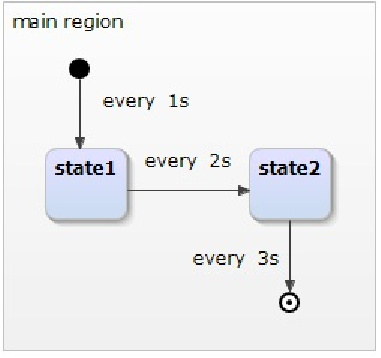
\includegraphics[width=55mm,scale=.55]{styles/simpleStateChart.pdf}}
	\label{simple_stateChart}
	\caption{Simple UML State Chart}
\end{figure}

The following are the basic notational elements that can be used to make up a diagram represented in figure \ref{simple_stateChart}:
\begin{itemize}
	\item Filled circle, representing to the initial state.	
	\item Hollow circle containing a smaller filled circle, indicating the final state (if any).	
	\item Rounded rectangle, denoting a state.	
	\item Arrow, denoting transition.	
\end{itemize}

Statechart diagram is used to describe the states of different objects in its life cycle. So the emphasis is given on the state changes upon some internal or external events. These states of objects are important to analyze and implement them accurately. Following are the main purposes of using Statechart diagrams:

\begin{itemize}
	\item To model dynamic aspect of a system.
	
	\item To model life time of a reactive system.
	
	\item To describe different states of an object during its life time.
	
	\item Define a state machine to model states of an object.
\end{itemize}

A set of formal representation of UML state charts is presented in this section. The state identifier and event are represented as S and Event respectively both as set types. For simple specification, the basic set types are used. In the definition of a transition from one state to another the guard is defined as a Boolean type. According to F Alhumaidan state based static and dynamic formal analysis of UML state diagrams \cite{ref_16_alhumaidan2012state} , a state can have three possible values that are active, passive or null represented as Active, Passive and null respectively. The type of state can be simple, concurrent, non-concurrent, initial or final.

\begin{figure}[ht!]
	\centering
	\begin{tabular}{lll}
		\footnotesize                       
		\textit{[S, Event]}          &\footnotesize \\
		
		\footnotesize
		\textit{Boolean}            &\footnotesize $::=$         &\footnotesize \textit{True} $\ \vert $ {False};       \\   
		\footnotesize
		\textit{Status}            &\footnotesize $::=$         &\footnotesize \textit{Active}
		 $\ \vert $ {Passive}$\ \vert $ {Null};       \\ 
		\footnotesize
		\textit{Type}            &\footnotesize $::=$         &\footnotesize \textit{Simple}
		 	$\ \vert $ {Concurent}$\ \vert $ {Nonconcurent} $\ \vert $ {Initial}$\ \vert $ {Final};       \\	 	 
		
	\end{tabular}
	\caption{UML Statechart Formal Representation}
	\label{statechart_formal_representation}
\end{figure}

In modeling using sets, it's not imposing any restriction upon the number of elements and a high level of
abstraction is supposed. Further, it's not insist upon any
effective procedure for deciding whether an arbitrary
element is a member of the given collection or not. As a
consequent, sets S and Event are sets over which cannot define any operation of set theory. For example,
cardinality to know the number of elements in a set cannot
be defined. Similarly, the subset, union, intersection or
complement operations over the sets are not defined.\\

The state diagram is a collection of states related by
certain types of relations. In the definition of a state, state identifier, its type, status and set of regions is required.Region is defined as a power set of sequence of states. The state is represented by a schema which consists of four components described above. All these components are encapsulated and put in the Schema State given below.
The invariants over the schema are defined in the second
part of schema.\\

\begin{figure}[ht!]
	\centering
	\begin{tabular}{lll}
		\footnotesize                       
		\textit{State}       \\
		
		\footnotesize
		\textit{name}   $:$    \textit{S}  \\   
		\footnotesize
		\textit{type}   $:$    \textit{Type}  \\   
		\footnotesize
		\textit{status}   $:$    \textit{Status}      \\
		\footnotesize
		\textit{regions} $:$   \textit{seq Regions} \\
		
		\footnotesize
		\textit{regions} $=$   \textit{1} $\ \  $ {type}$=$   \textit{Simple} \\
		\footnotesize
		 \textit{\# regions} $=$   \textit{1} $\ \  $ {type}$=$   \textit{Nonconcurrent} \\
		 \textit{\# regions} $=$   \textit{1} $\ \  $ {type}$=$   \textit{Concurent} \\
		 
		
	\end{tabular}
	\caption{UML statechart some other formal representation}
	\label{statechart_formal_representation_part2}
\end{figure}

\textbf{Invariants:}
\begin{itemize}
\item  If there is no region in a state inside the state diagram, then it is a simple state.
\item  If there is exactly one region in a state then it is termed as non-concurrent composite state.
\item  If there are two or more regions in a state then it is
concurrent composite state.
\end{itemize}

The collection of states is represented by the schema
States which consists of four variables. The mapping
substates from State to power set of State describes type
of a state.
 \begin{figure}[ht!]
 	\centering
 	\begin{tabular}{lll}
 		\footnotesize                       
 		\textit{States}          \\
 		\footnotesize                       
 		\textit{start}          
 		$:$  \textit{State}\\
 		
 		\textit{states}          
 		$:$  \textit{State}\\
 		
 		\textit{states}           
 		$:$  \textit{State}\\
 		\footnotesize
 		\textit{substates}            $:$         \textit{State} $\ \  $ {State};       \\   
 		\footnotesize
 		\textit{target}             $:$         \textit{State}    \\
 		 \footnotesize                       
 		 \textit{start}           
 		 $:$  \textit{states}\\
 		  \footnotesize                       
 		  \textit{start}          
 		  $:$ \textit{target}\\
 		   \footnotesize                       
 		   \textit{start}           
 		   $:$  \textit{dom} $\ \  ${substates}\\
 		   
 		   \footnotesize                       
 		   \textit{states}          \\ 		
 		$\ \  $ \textit{s}      $:$     \textit{State} $\ \  $ {s} $\ \  $ \textit{dom} $\ \  ${substates} $\ \  $ {s} $\ \  $ \textit{states}        \\ 
 		$\ \  $ \textit{s}      $:$     \textit{State} $\ \  $ {s} $\ \  $ \textit{states} $\ \  $ {s} $\ \  $ \textit{start} $\ \  $ {s} $\ \  $ \textit{target}$\ \  $ {s.typ}\\ 
 		$\ \  $ \textit{Simple} $\ \  $ {s} $\ \  $ \textit{dom} $\ \  ${substates}\\
 		\footnotesize                       
 		\textit{target}  $\ \  $ \textit{states}        \\ 
 		\footnotesize                       
 		\textit{target}  $\ \  $ \textit{dom} $\ \  ${substates}\\	
 	\end{tabular}
 	\caption{UML Statechart Formal Representation some parts}
 	\label{statechart_formal_representation_invariants}
 	\end{figure}

\textbf{Invariants:}
\begin{itemize}
\item The start state is not in the collection of states.
\item The start state is not the target state.
\item The start state does not belong to domain of substates
mapping that is it has no sub-state.
\item The set of states is non-empty.
\item For any state, s, if it is in the states and is not the start or target state and not the simple state then it belongs to domain of sub-states.
\item The target state does not belong to states.
\item The target state of the state diagram does not belong to domain of the sub-states.
\end{itemize}

UML state chart editor has been extended based on the open source Yakindu SCT \cite{ref_15_yakindu:sct}framework. The existing language grammar with
annotation language grammar has extended in order to support new set
of tags. Furthermore, an annotation proposal filter implemented which was used to filter out the annotation language tags of the Yakindu SCT language grammar.\\

To extend the Yakindu SCT editor here it has been decided to represent the statements like variable declaration, function calling as state and transitions are represent as move from one statement to another. A rectangular box can be attached with transitions where annotation can be written as per requirements. So for the developed system the UML statechart formal representation is as like this: 
\begin{figure}[ht!]
	\centering
	\begin{tabular}{lll}
	\footnotesize                       
	\textit{States}          \\
	\footnotesize                       
	\textit{start}          
	$:$  \textit{State}\\
	
	\textit{states}          
	$:$  \textit{State}\\
	
	\textit{states}           
	$:$  \textit{State}\\
	\footnotesize
	\textit{substates}            $:$         \textit{State} $\ \  $ {State};       \\   
	\footnotesize
	\textit{target}             $:$         \textit{State}    \\
	\footnotesize                       
	\textit{start}           
	$:$  \textit{states}\\
	\footnotesize                       
	\textit{start}          
	$:$ \textit{target}\\
	\footnotesize                       
	\textit{transition}          
	$:$ \textit{annotation*}\\
	\footnotesize                       
	\textit{target} $:$ \textit{states}        \\ 	
	\end{tabular}
	\caption{UML Statechart Formal Representation for this System}
	\label{statechart_formal_representation_for _this_system}
	\end{figure}
\section{Source Code Editor}
The source code editor has extended which offers annotation language proposals which are context sensitive with respect to the position of the currently edited syntax line. Editor suggestions work only if the whole file is parsed without errors. Editor was developed using Eclipse Xtext \cite{ref_17_xtext:grammar}.

As per requirements previous annotation language grammar which was written in xtext language has been extended. Extra annotation have included like \enquote{authenticated}, \enquote{declassified}, \enquote{sanitized}, \enquote{sanitization}, \enquote{declassification}, \enquote{authentication}. Mainly FunctionAnnotation, FunctionType  and SingleLineAnnotation rules  are extended. A new rule is added which is enumeration type. The rule name is VariableType. Inside the VariableType new attributes are included like declassified, sanitized and authenticated. New function types are added like declassification, sanitization and authentication function inside FunctionType rule. Inside the FunctionAnnotation and SingleLineAnnotation rules there exist an annotation for parameter name @parameter. Inside @ parameter declaration new attribute is added named VariableType. Some part of the code snippet of extended xtext grammar is given below. 

\begin{lstlisting}
/**
* @FunctionAnnotation :used for function annotations
*/ 
FunctionAnnotation returns FunctionAnnotation:
{FunctionAnnotation}( 
result +=  '@function '   functionType=FunctionType      (' ')?                              (level =('H'|'L'))?     ((name0=ID))? ((nameComment=ID))? ('\n' | '\r')?
// supported without space before confidential and sensitive
| '@parameter '   parameter=ID (name0=ID)? (securityType=SecurityType)?(' ')?  (level =('H'|'L'))? ('True'|'False')? (variableTyp=VariableType)?  ((name1=ID))? ((nameComment=ID))? ('\n' | '\r')?	
;

/**
* @SingleLineAnnotation :used for adding single line annotations
*/ 
SingleLineAnnotation returns SingleLineAnnotation:
{SingleLineAnnotation}(
result+=  '//@ @function '    functionType=FunctionType (' ')?                  (level =('H'|'L'))?  ((name0=ID))? ((nameComment=ID))?  ('\n' | '\r')*
// supported without space before confidential and sensitive
| '//@ @parameter '   parameter=ID (securityType=SecurityType)? (' ')?  (level =('H'|'L'))? ('True'|'False')? (variableTyp=VariableType)?  ((nameComment=ID))?  ('\n' | '\r')?
| '//@ @variable '    variable=ID  (securityType=SecurityType)? (' ')?  (level =('H'|'L'))? ('True'|'False')? ((nameComment=ID))?  ('\n' | '\r')?

;

/**
* @FunctionType :annotaions types for functions
*/ 
enum FunctionType: declassification 
| sanitization
| authentication
| sink
| source
| trust_boundary
;


/**
* @Variable Type :annotaions types for function parameters
*/ 
enum VariableType: declassified 
| sanitized
| authenticated
;	
\end{lstlisting}

From the above xtext code snippet previous annotation grammar has FunctionAnnotation, SingleLineAnnotation rules. According to the requirements previous rules are extended. Inside the rules of FunctionAnnotation and SingleLineAnnotation new enumeration types are added. Enumeration type name is VariableType. The new enumeration type rule has attributes declassified, sanitized and authenticated. Also the rule of enumeration FunctionType extended by adding new type of funtion like authentication, declassification and sanitization.

\section{C Code Generator}
C code generator has extended based on Eclipse EMF and xTend which is used to generate the state chart execution code containing the previously added security annotations from UML state charts. The code generator outputs two files per UML state chart (one .c and one
.h file). Generated annotations can reside in both header file
and source code file. Previously annotated UML state chart
states are converted to either C function calls or C variables
declarations, both have been previously annotated. We use
the available state chart execution flow functionality which is
responsible for traversing the UML state chart during state
chart simulation. The UML state chart will be traversed by the code generation algorithm and code is generated based on
the mentioned state chart execution flow. The generated code
will contain at least one bad path (contains a true positive) and
a good path (contains no bug) per UML state chart if those
paths were previously modeled inside the UML state chart.\\

The algorithm is given below how the C code generator has been created. The input of the algorithm for code generator is UML statechart. In eclipse xtend \cite{ref_20_xtend} function can be declared as \enquote{def}. Here the generateTypeH function requires the input of UML statechart. The plug-in named \enquote{MyC} uses eclipse xtend to parse the UML statechart. Inside this function there another two functions named \enquote{typesHAnnotationContent} to generate header file of c(extension .h) and \enquote{typesCAnnotationContent} to generate source code file of c(extension .c).Function typesHAnnotationContent generate the required contents for C header file mostly function signature and annotation of the function which exist in the UML statechart. One sample example of a header file is given below-

\begin{lstlisting}
	/*@ @function authentication
	* @parameter a L @*/
	void authentication(char *a);
	
	/*@ @function source
	* @parameter a L @*/
	void logIn(char *a);
\end{lstlisting}

Function typesCAnnotationContent generate the required contents for C source file. This file contains the annotation only for variable declaration. The function annotation is normally located at header file. In this file other code is as normal as C syntax. All functions,statements, variable declaration ar similar to C programming language syntax. Some of the contents of the C file comes from another xtend file named \enquote{Naming.xtend} which contains in \enquote{MyC} project folder of YAKINDU Sct Editor. some part of code snippet from \enquote{Naming.xtend} file is given below:

\begin{algorithm}
	{\textbf{C code generator}}\\
	\noindent\makebox[\linewidth]{\rule{\textwidth}{0.4pt}}
	{\textbf{Input: Statechart}} \\
	{\textbf{Output: .c and .h files}}
	\begin{algorithmic}[1]
	
		\Function{generateTypesH}{$sc$}\Comment{Where sc - statchart}
		
			\State $def {generateFile_1} (testModule.h, typesHAnnotationContent(sc)) $ {Where def - function declaration in xtend}
			\State $def {generateFile_2} (testModule.c, typesCAnnotationContent(sc)) $
		\EndFunction
		
		\Function {typesHAnnotationContent}{$sc$}		
			\For{$s : getFileContent(sc).entrySet$}
				\If {$!s.key.contains('//@ @variable')$}
					\State $s.key$
				\ElsIf {$s.value.contains('(')$}
					\State $ void <s.value>;$
				\EndIf		
			\EndFor			
		\EndFunction
		
		\Function {typesCAnnotationContent}{$sc$}
		
		\For{$s: getFunctionContent(sc).entrySet$}
			\If {$(!s.value.contains('authentication') and (!s.value.contains('declassification'))$  \\  
			$\   \   $   $and(!s.value.contains('sanitization')))$}
				\State $void <s.value> {}$
			\EndIf		
		\EndFor
			
		\For{$ region : sc.regions$}
			\If {$ region.name.equalsIgnoreCase('bad_path()'$}
			\State $void <region.name>$
				
					\For {$s: getBadPathContent(sc).entrySet$}
					
						\If {$ s.key.contains('//@ @variable')$} 
							\State $s.key$
							\State $s.value$
						\EndIf
					
						\If {$ s.value.contains('(')$} 
							\State $s.value;$
							\State $s.value$
						\EndIf
					
					\EndFor 
			\EndIf
		
			\If {$ region.name.equalsIgnoreCase('good_path()')$} 
			\State $void <region.name>$
				\For {$s: getGoodPathContent(sc).entrySet$}
					\If {$s.key.contains('//@ @variable')$} 
						\State $s.key$						
					\EndIf
					\State $s.value;$
				\EndFor 
			\EndIf
				
		\EndFor
				
		\EndFunction
		
		
	\end{algorithmic}
	\noindent\makebox[\linewidth]{\rule{\textwidth}{0.4pt}}
\end{algorithm}

Below from the xtend code snippet it can be seen that from the state chart xtend can easily accessible the contents of the state chart which is designed in the modeling stage. For example in case of the function \enquote{getFunctionContent} it parses the function names and put it inside a hash map. It parses those as a function who is a state and contains first bracket like "(". Inside the hashmap it puts the function name and function annotation. In case of the function \enquote{getBadPathContent} which returns the content for the bad path. From the content of state chart there is a region which named is "bad\_path()". From that region this function parses the comments from each transition and gets the name of each state. Then it puts those contents into a hash map. Through iterating that map according to the algorithm it puts some part of contents in C header file and some part in source code file. The purpose of function \enquote{getGoodPathContent} is to get all the required content from the good path(which is not buggy path). The parameter of this function is the state chart. In the modeling phase it has been declared as a region named "good\_path()". This \enquote{getGoodPathContent} function starts parsing the contains from good path then traverse the whole good path and get all the required contents. After that this function puts the content into a hash map. This hashmap also contains the function name, function annotation, variable declaration which has annotation. Then according to the algorithm by iterating through the hash map generates the required files by putting the contents in proper place. \\

\begin{lstlisting}
	def HashMap<String, String> getFileContent(Statechart sc) {	
		var fileContent = <String, String>newHashMap
		for( region : sc.regions){
			for(vertex : region.vertices)  {
				if (!(vertex.name.nullOrEmpty)){
					for(transition : vertex.incomingTransitions) {
						fileContent.put(transition.specification,vertex.name)			
					}							
		
				}
		
			}     
		
		}          
	return fileContent
	}
	
	def HashMap<String, String> getFunctionContent(Statechart sc) {
		var functionContent = <String, String>newHashMap	
		for( region : sc.regions){	
			for(vertex : region.vertices.filter[eClass.name.contentEquals('State')])  {	  
	
				if ( (vertex.name.contains('(')) && (!(vertex.name.nullOrEmpty))){						
					functionContent.put(vertex.name,vertex.name)
				}
			}    
		}          
		return functionContent
	}
	
	def HashMap<String, String> getBadPathContent(Statechart sc) {
		var badfunctionContent = <String, String>newHashMap
		var String newName
	
			for( region : sc.regions){
	
				if(region.name.equalsIgnoreCase('bad_path()')){
					for(vertex : region.vertices.filter[eClass.name.contentEquals('State')]){			
	
						if(!(vertex.name.contains('(')) && (!(vertex.name.nullOrEmpty))){
							for(transition : vertex.incomingTransitions) {
							badfunctionContent.put(transition.specification,vertex.name)			
							}							    
						}
						if((vertex.name.contains('(')) && (!(vertex.name.nullOrEmpty))){
							if ( (vertex.name.contains('char '))){
								newName=vertex.name.replaceAll('char *','')
								if(newName.contains('*'))	
									newName=newName.replaceAll('\\*',''		)				
								badfunctionContent.put(newName,newName)
								}
							else
								badfunctionContent.put(vertex.name,vertex.name)
						}
					}
	
				}     
	
			}          
		return badfunctionContent
	}
	
	def String getVariableName(Statechart sc){		
		var String variablename
			for( region : sc.regions){
				for(vertex : region.vertices.filter[eClass.name.contentEquals('State')])  {	 
	
					if (!(vertex.name.contains('(')) && (!(vertex.name.nullOrEmpty))){						
						for(transition : vertex.incomingTransitions) {												
							variablename= vertex.name.replaceAll('char *','')
							if(variablename.contains('*'))
							variablename=variablename.replaceAll('\\*','')														
						}
					}
				} 
	
			}
		return variablename
	}
	
	def HashMap<String, String> getGoodPathContent(Statechart sc) {
		var goodfunctionContent = <String, String>newHashMap	
		var String newName		
	
			for( region : sc.regions){
					if(region.name.equalsIgnoreCase('good_path()')){
	
							val choiceState=0; 
							val increment=1; 
	
							for(vertex : region.vertices.filter[eClass.name.contentEquals('Choice')]){                   	
									val sum=choiceState+increment;
									for(transition : vertex.incomingTransitions) {                	
										System.out.println("*********"+"if\n"+sum);     
	
									}         	    
							}
	
							for(vertex : region.vertices.filter[eClass.name.contentEquals('State')])  {			    
	
	
									for(invertex : vertex.parentRegion.vertices.filter[eClass.name.contentEquals('State')])
										{
												if(!(vertex.name.contains('(')) && (!(vertex.name.nullOrEmpty))){
														for(transition : vertex.incomingTransitions) {
																goodfunctionContent.put(transition.specification,vertex.name)
	
														}
												}
												if((vertex.name.contains('(')) && (!(vertex.name.nullOrEmpty))){
	
														if ( (vertex.name.contains('char '))){
	
																newName=vertex.name.replaceAll('char *','')	
																newName=newName.replaceAll('\\*','')					
																goodfunctionContent.put(newName,newName)
																}
																else
																goodfunctionContent.put(vertex.name,vertex.name)
																}
	
								}
	
	
						} 
		
				}    
	
			}          
		return goodfunctionContent
	}	

\end{lstlisting}






\section{Three Checkers in Static Analysis Engine}
Static analysis refers analyzing code without executing it. Generally it is used to find bugs or ensure conformance to coding guidelines. The classic example is a compiler which finds lexical, syntactic and even some semantic mistakes.Static analysis tools should be used when they help maintain code quality. If they're used, they should be integrated into the build process, otherwise they will be ignored.Some characteristics of static analysis tools are:
\begin{itemize}	
	\item Identify anomalies or defects in the code.
	\item Analyze structures and dependencies.
	\item Help in code understanding.
	\item To enforce coding standards.
\end{itemize}

For this system static analysis engine \enquote{smtcodan}  has been used. Inside the engine to detect the information flow vulnerabilities required classes like AuthenticationFunctionChecker.java, DeclassificationFunctionChacker.java, SanitizationFunctionChecker.Java, Authentication\_gen.java,\\
Declassification\_gen.java,
Sanitization\_gen.java files are included. These files are included in order to detect authentication, declassification and sanitization function missing bug detection in C code. For these three types of function detection here it has been used as library functions in C programming language. In order to detect the information flow vulnerabilities three models have been included such as Authentication\_gen.java,
Declassification\_gen.java,
Sanitization\_gen.java. In the generated .c file there exist these three kinds of methods without signature which is given in figure . As they have no method body that's why they are acting as library function in \enquote{smtcodan} static analysis engine. Inside the engine three function signature will act as keyword like authentication, declassification and sanitization function. \\

From C code generator generated .c and .h file with annotation should act as input for \enquote{smtcodan} static analysis engine. Engine parses the code with annotation. The authentication, declassification and sanitization function all makes the high secured variable or confidential variable as low and according to the policy they passes the information from the sender to the receiver in a secured way. While implementing the checkers, information flow restriction has followed. If any of the C files are not following the secure information flow then bug should be triggered as either authentication , declassification or sanitization function missing function.

\section{View Buggy Path in Sequence Diagram}

The Sequence Diagram models the collaboration of objects based on a time sequence. It shows how the object's interact with others in a particular scenario of a use case.A popular use for them is to document the dynamics in an object-oriented system. For each key collaboration, diagrams are created that show how objects interact in various representative scenarios for that collaboration.An important characteristic of a sequence diagram is that time passes from top to bottom : the interaction starts near the top of the diagram and ends at the bottom. Some of the components of sequence diagram \cite{ref_107_visual-paradigm:visual-paradigm} is described below-

\begin{itemize}
	\item \textbf{Actor:} An Actor models a type of role played by an entity that interacts with the subject (by exchanging signals and data), but which is external to the subject (in the sense that an instance of an actor is not a part of the instance of its corresponding subject). Actors may represent roles played by human users, external hardware, or other subjects. Note that an actor does not necessarily represent a specific physical entity but merely a particular facet (role) of some entity that is relevant to the specification of its associated use cases. Thus, a single physical instance may play the role of several different actors and, conversely, a given actor may be played by multiple different instances.
	
	\item \textbf{Call Message:} A message defines a particular communication between Lifelines of an Interaction. Call message is a kind of message that represents an invocation of operation of target lifeline.
	
	\item \textbf{Create Message:} A message defines a particular communication between Lifelines of an Interaction. Create message is a kind of message that represents the instantiation of (target) lifeline.
	
	\item \textbf{Destroy Message:} A message defines a particular communication between Lifelines of an Interaction. Destroy message is a kind of message that represents the request of destroying the lifecycle of target lifeline.
	
	\item \textbf{Duration Message:} A message defines a particular communication between Lifelines of an Interaction. Duration message shows the distance between two time instants for a message invocation.
	
	\item \textbf{Found Message:} A found message is a message where the receiving event occurrence is known, but there is no (known) sending event occurrence. 
	
	\item \textbf{LifeLine:} A lifeline represents an individual participant in the Interaction.
	
	\item \textbf{Lost Message:} A lost message is a message where the sending event occurrence is known, but there is no receiving event occurrence. We interpret this to be because the message never reached its destination.
	
	\item \textbf{Message:} A message defines a particular communication between Lifelines of an Interaction.
	
	\item \textbf{Return Message:} A message defines a particular communication between Lifelines of an Interaction. Return message is a kind of message that represents the pass of information back to the caller of a corresponded former message.
	
	\item \textbf{Note:} A note (comment) gives the ability to attach various remarks to elements. A comment carries no semantic force, but may contain information that is useful to a modeler.
	
	\item \textbf{Send Message:} A message defines a particular communication between Lifelines of an Interaction. Send message is a kind of message that represents the start of execution.
	
	\item \textbf{Sequence Message:} A message defines a particular communication between Lifelines of an Interaction. Sequence message is a kind of message that represents the need of performing actions in sequence.
	
	\item \text{Frame:} A frame represents an interaction, which is a unit of behavior that focuses on the observable exchange of information between ConnectableElements.
	
	\item \textbf{Concurrent:} A concurrent represents a session of concurrent method invocation along an activation. It is placed on top of an activation.
	
	\item \textbf{Constraint:} A condition or restriction expressed in natural language text or in a machine readable language for the purpose of declaring some of the semantics of an element.
	
	\item \textbf{Continuation:} A Continuation is a syntactic way to define continuations of different branches of an Alternative CombinedFragment. Continuation is intuitively similar to labels representing intermediate points in a flow of control.
	
	\item \textbf{Gate:} A Gate is a connection point for relating a Message outside an InteractionFragment with a Message inside the InteractionFragment.
	
	\item \textbf{Alternative Combined Fragment:} A combined fragment defines an expression of interaction fragments. A combined fragment is defined by an interaction operator and corresponding interaction operands. Through the use of CombinedFragments the user will be able to describe a number of traces in a compact and concise manner.
	
	\item \textbf{Recursive Message:} A message defines a particular communication between Lifelines of an Interaction. Recursive message is a kind of message that represents the invocation of message of the same lifeline. It's target points to an activation on top of the activation where the message was invoked from.
	
	\item \textbf{Self Message:} A message defines a particular communication between Lifelines of an Interaction. Self message is a kind of message that represents the invocation of message of the same lifeline.
	
	\item \textbf{Terminate Message:} A message defines a particular communication between Lifelines of an Interaction. Terminate message is a kind of message that represents the termination of execution.
	
	\item \textbf{Interaction Use:} An InteractionUse refers to an Interaction. The InteractionUse is a shorthand for copying the contents of the referred Interaction where the InteractionUse is. To be accurate the copying must take into account substituting parameters with arguments and connect the formal gates with the actual ones.
	
	\item \textbf{Time Constraint:} A TimeConstraint defines a Constraint that refers to a TimeInterval.
	
	\item \textbf{Uninterpreted Message:} A message defines a particular communication between Lifelines of an Interaction. Uninterpreted message is a kind of message that represents an uninterpreted call.
	
	\item \textbf{Return Message:} A message defines a particular communication between Lifelines of an Interaction. Return message is a kind of message that represents the pass of information back to the caller of a corresponded former message.
	
	\item \textbf{Note:} A note (comment) gives the ability to attach various remarks to elements. A comment carries no semantic force, but may contain information that is useful to a modeler.	
	
\end{itemize}

In this research we used sequence diagram to view the buggy path. In our case the sending messages are function call. One function call used to move from one lifeline to another lifeline. We used statements(with line number and file name) before function call into the lifeline which will help the user to view the buggy path easily.

Through the static analysis engine buggy path can be found as a list of string. Inside the list there are function calls, separate statements like if statements, switch-case statements, variable declaration, assignment of variables etc. of programming language (like C,C++). Then to view the path using java a sequence diagram is generated. Inside the sequence diagram all function calls are included inside rectangular box attached to the head of timeline. To switch one timeline to another a function call required. Like in the figure \ref{Error_trace_path} from function call int main() there is a transition to move from int main() to good\_path(). Above the transition there also exist the function name for which it goes from one function call to another. Here for example to move from int main() to good\_path() there is a transition and above that transition function call good\_path() is attached. This means through calling the good\_path() function buggy path goes into good\_path() function from int main(); Inside the sequence diagram the statements before the function call are attached to the timeline as blue color. Those statements are just the statements before a function of the analyzed C/C++ source code file. Inside the box of the blue color texts there exist "ln:" which means the line number of the statement in the analyzed file and "fn:" means the file name of analyzed file.Now it is easier to trace the buggy path by viewing generated sequence diagram.

 One sample example of the part of a buggy path is given in figure \ref{Error_trace_path}.
\begin{figure}[htbp]
	\centering
	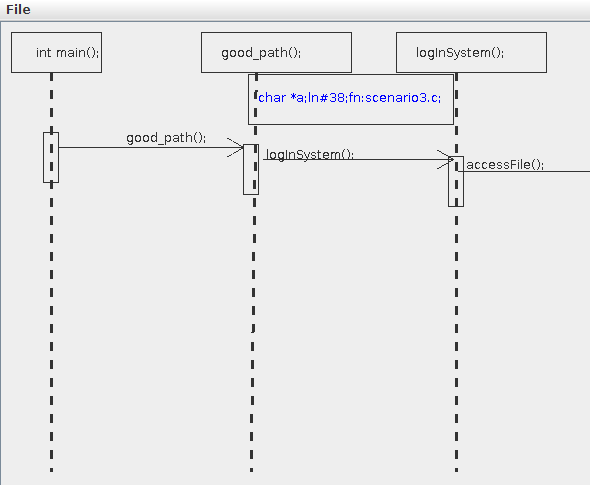
\includegraphics{styles/error_trace_path.png}
	\label{Error_trace_path}
	\caption{Error trace path in UML sequence diagram}
\end{figure}

The process of creating sequence diagram using Java programming language is given below as an algorithm representation. To develop the sequence diagram a separate class is included inside the smtcodan project. The class name is SequenceDiagramGenerator. Inside this class the drawSequenceDiagram function creates the diagram. The function input parameter is a list of IASTNode which is delivered from the smtcodan project packages. To draw the diagram BufferedImage, Graphics2D, JPanel, JFrame  classes were used. At first need to declare object each of these(BufferedImage, Graphics2D, JPanel, JFrame) classes. Then iterating through the list of IASTNodes set all the statements except function call with line number and file name. There is a class which is responsible to draw the visual things of the sequence diagram named MyCanvasDraw. Afterwards need to create an object of this class. This class has a list. The list of this class has to be set with the list of all statements, line number  and file name. Then it will draw the diagram according to the list. To view this diagram need to set the JFrame object and make it visible. Inside the JFrame JScrollpane object also added to make the frame scrollable. For saving the diagram as an image save as option also included. Through the menu bar user can easily save the sequence diagram as an image. By default it will save the image as in .jpg format. But one can easily save this image in other format like .png,.bmp,.jpeg etc. Exit option is also included inside the JFrame through which user can exit the current window.  


\begin{algorithm}
	{\textbf{Sequence diagram generator}}\\	
	\noindent\makebox[\linewidth]{\rule{\textwidth}{0.4pt}}
	{\textbf{Input: List of statements and function call}} \\
	{\textbf{Output: Sequence diagram in a Jframe}}
	\begin{algorithmic}[1]
		
		\Function{drawSequenceDiagram}{$ArrayList<IASTNode> statementsList$}
		    \State $ frame  <- JFrame  $ 
			\State $ image  <- BufferedImage  $ 
			\State $ graphics2D  <- Graphics2D  $
			\State $ topPanel <- JPanel $
			\State $ mcd <- MyCanvasDraw $
			\For{$i:statementsList.size()$} 
				\If {$!statementsList.get(i).getRawSignature().toString().contains("(")$}
					
					\State $int j=i;$
					\If{$j<=statementsList.size()-2$}
						\State $do$
						\State $add(line number)$
						\State $add(file name)$
						\State $while(!statementsList.get(j).getRawSignature().toString().contains("("))$
						\State $mcd.buggyPathList.add(allStatements);$ \Comment{Where allStatements - statements with containing line number and file name also}
					\EndIf				
				\EndIf		
				
			\EndFor
				\State $set <- JScrollPane(property)$
				\State $mcd.paint(graphics2D)$
				\State $topPanel.add(mcd);$	
				\State $menuBar <- JMenuBar$
				\State $menuFile <- JMenu $
				\State $menuFileExit <- JMenuItem$
				\State $menuSaveAs <- JMenuItem $
				\State $menuSaveAs.addActionListener <- fileSave and exit$
				\State $set<-frame (properties=visibility,menubar)$
		
		\EndFunction		
		
	\end{algorithmic}
	\noindent\makebox[\linewidth]{\rule{\textwidth}{0.4pt}}
\end{algorithm}
